\chapter{Introduction}

\section{Camera systems}
\section{Scientific camera systems}
\section{X-band scientific grade cameras}
\subsection{Scintillation cameras}
\subsection{Silicon sensor cameras}

%\section{Framework definition}
%%system subsystem component diagram 
%
%\section{Camera architecture}
%    \subsection{Basics}
%    \subsection{Electronics}
%    \subsection{Mechanics}
%    \subsection{Firmware}
%
%\section{Review of existing camera design frameworks}
%
%\section{Embedded system design on novel SoC}
%\subsection{Digital system (Xilinx) }
%
%    Xilinx Vivado software is used for development on Zynq SoC devices. There are two ways to design a digital system
%    in Vivado, by writing VHDL and by creating a block design. Pure VHDL allows for creating standard processes, state
%    machines etc., whereas block design is a graphical interface for configuring and connecting IP Cores together.  
%    The design is done on a higher level of abstraction (top-down design\ref{DIGSYS:TOP_DOWN}). Created block design is
%    wrapped into a wrapper which then can be added to the top design file. Multiple block design
%    can be present in one project. 
%
%        \begin{figure}[h!]
%          \centering
%          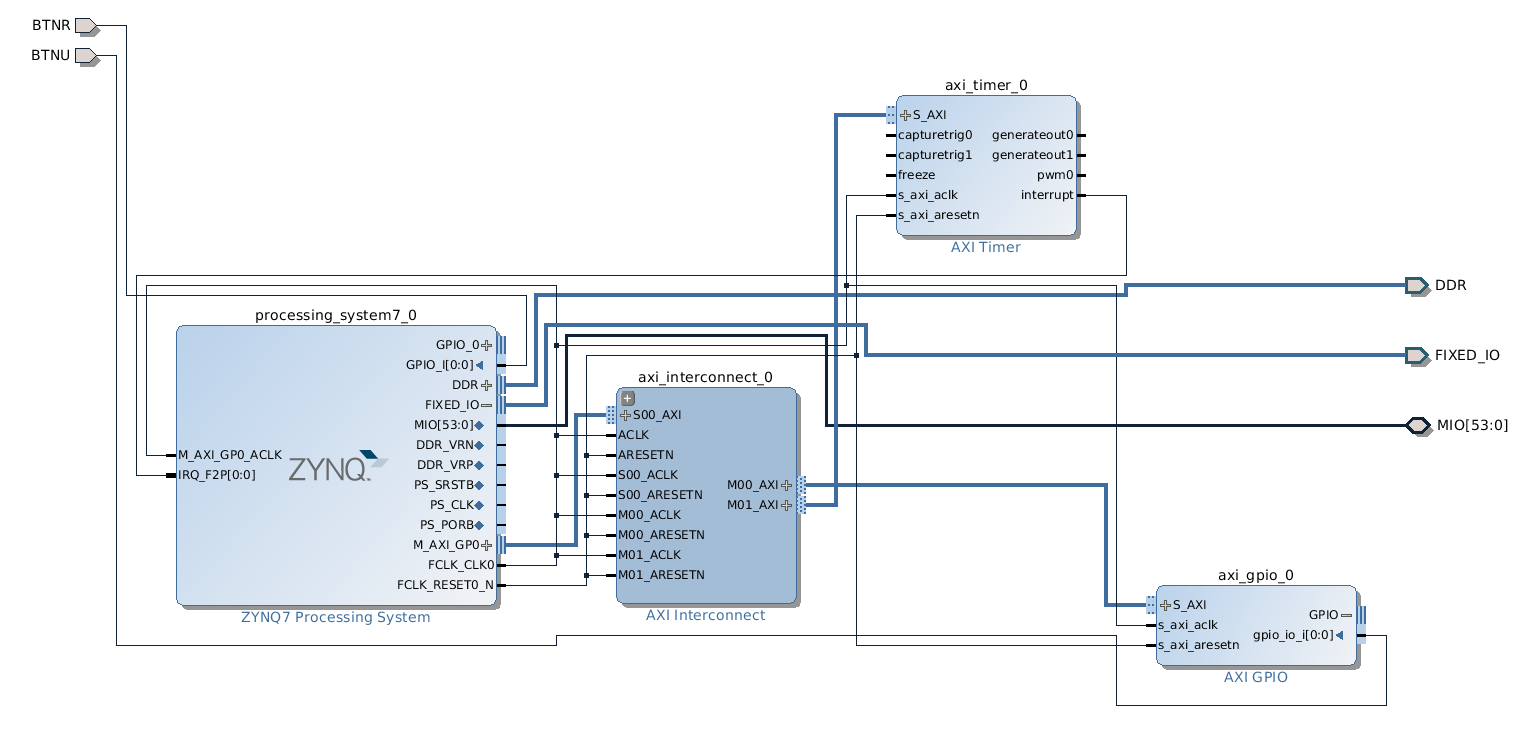
\includegraphics[width=13cm]{img/realisation/block_design.png}
%          \caption{ An example of a block diagram}
%          \label{FIG:BLOCK_DES}
%        \end{figure}
%
%\subsection{}
%
%\section{Literature review}
%    \subsection{Scientific research}
%
%\
%@book{BOOK:MULTI_CAMERA,
%    author    = "Hamid Aghajan, Andrea Cavallaro",
%    title     = "Multi-Camera Networks: Principles and Applications",
%}
%
%@book{BOOK:PROGRAMMING_EMBEDDED,
%    author    = "Christophe Bobda, Senem Velipasalar",
%    title     = "Programming Embedded Systems in C and C++",
%}
%
%@book{BOOK:DISTRIBUTED,
%    author    = "by Christophe Bobda, Senem Velipasalar",
%    title     = "Distributed Embedded Smart Cameras: Architectures, Design and Applications",
%}


%
%One cannot deny the fact that one of the most important aspects of any project is development time.
%This is both relevant to commercial market and scientific research, where a possibility to quickly test a 
%hypothesis and build a prototype is invaluable. In specialised industries, the possibility to quickly adjust the 
%parameters of a specific system suited to the customer's needs is a key to success. Sometimes, even a worse product can 
%win on the market simply because it was released earlier.  
%
%The following master thesis presents a firmware for scientific camera systems. The purpose of the thesis is
%to ease design and shorten development time of a scientific camera. There are no such open frameworks available
%for use by the scientific community. Although, commercial products are available, they do not provide enough
%flexibility. Thus the camera design framework is presented to fill this gap. 
%
%The thesis is divided into 5 chapters. The first chapter describes the scientific camera design, the theory and
%current state of technology, and also the reasons for doing this work. Chapter 2 contains the requirements of the Camera
%framework. The third chapter presents the concept phase of the project, where the main project decisions are made. 
%After the concept chapter, the realisation and tests are described in Chapter 4. 
%In the end, the whole project is summarised in Chapter 5.
%
%\section{Basics}
%
%A camera is an electro-mechanical device used for capturing images or videos. 
%The basic principle of the camera operation is common to all types. The visible light (or a portion of the electromagnetic
%spectrum) enters the camera box through a converging lens and records the image on a light-sensitive medium, like a
%photographic film or electronic sensor.  It consists of a few main parts: optics, 
%sensor, processing system, enclosure, buttons and communication interface and storage medium.
%Figure~\ref{fig:camera} presents the explanatory diagram of a digital camera.
%
%\begin{figure}[h!]
%    \centering
%    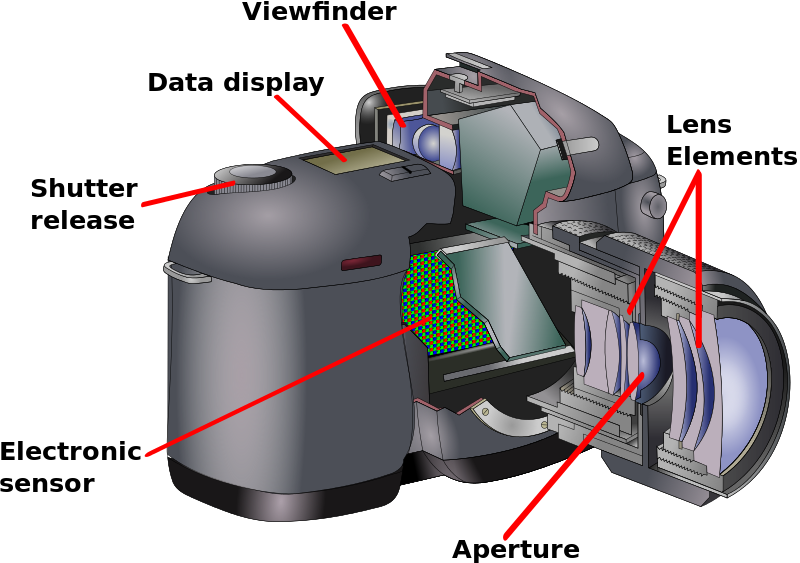
\includegraphics[width=13cm]{img/introduction/camera.png}
%    \caption{Basic digital camera diagram~\cite{PIC:CAMERA_DIAG}}
%    \label{fig:camera}
%\end{figure}
%
%In general, cameras have existed for over 170 years and digital ones for 25 years~\cite{BOOK:170YEARS_OF_CAMERAS}. They are used
%in every industry and market. They have changed humanity and allowed us to unveil new discoveries. 
%In general, cameras can be divided into many groups. One way is to distinguish consumer cameras (both
%professional and amateur) and scientific cameras. 
%
%Consumer cameras are used everyday by thousands of people. They are inexpensive and provide good quality pictures
%and videos. Almost every mobile phone has a camera which allows people to take photos whenever they want.
%What is more, the advanced devices like DSLR\footnote{Digital Single Lens Reflex} cameras provide much higher
%image quality and allow people to exchange the lens. They are used by amateur and professional photographers and video makers.
%
%Companies such as: Nikon~\cite{WWW:NIKON}, Canon~\cite{WWW:CANON} and Sony~\cite{WWW:SONY} provide products 
%which have certain parameters needed by consumers. The life cycle of a commercial
%camera is from one to two years. Each year, companies put new products on the market with new features and
%better parameters to keep their income stable. 
%
%The market of scientific cameras is different. The cameras used for telescopes, medical devices, and ADAS\footnote{Advanced
%driver assistance system} are of a different type than commercial ones. They do not focus on the wireless connectivity
%or ease of use, but only on performing one specific task in the best possible way. For example, telescope cameras 
%provide extremely high sensitivity and, in order to achieve this, the sensor is cooled down to low temperatures. This is 
%not comparable to commercial cameras.
%
%Their design is much more complex due to specific requirements like sensitivity or high speed operation. 
%Figure~\ref{fig:piofthesky} presents the scientific camera system used in \emph{$\pi$ of the sky project}~\cite{WWW:PI_OF_THE_SKY}. 
%The project is a sophisticated multichannel system consisting of 16 CCD cameras and used for detecting
%optical flashes accompanying Gamma Ray Bursts. 
%
%\begin{figure}[h!]
%    \centering
%    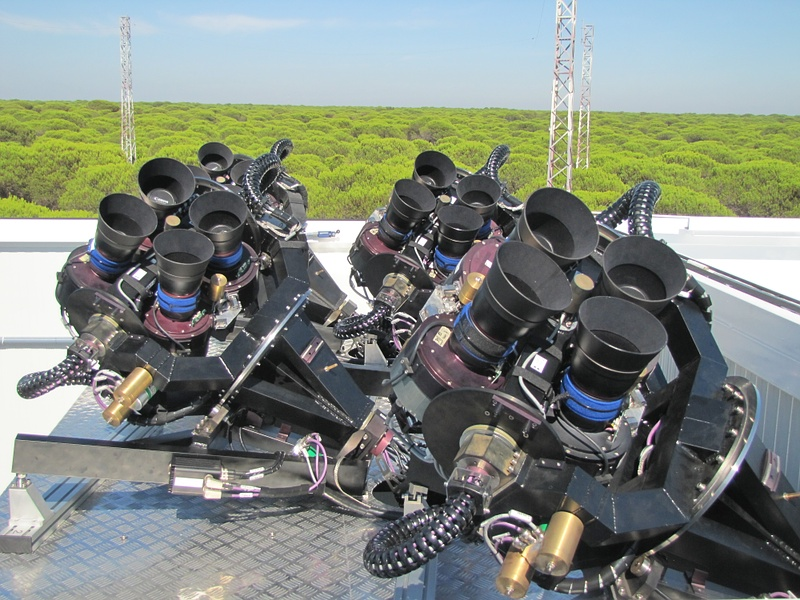
\includegraphics[width=13cm]{img/introduction/camera_pi.jpg}
%    \caption{$\pi$ of the Sky camera system~\cite{WWW:PI_OF_THE_SKY}}
%    \label{fig:piofthesky}
%\end{figure}
%
%%\section{The need for a specialised framework}\label{ch1:theory}
%%The complexity of the design of a camera system for commercial and scientific use is overwhelming. There is no    
%
%\section{Theory of camera design}\label{ch1:theory}
%%
%%This section introduces the topic of camera design.  Firstly, all the most important
%%subsystems of a camera are presented in detail. Next, the scientific camera design specifics are shown. Last section summarizes the chapter.
%
%From the software and digital system perspective, the camera is an embedded system whose main functions are acquiring
%image from the sensor, processing it, and storing or transmitting it for further processing. As simple as it sounds, this is a complicated task
%given today's sensors resolutions, required noise characteristics and other parameters. What is more,
%cameras for scientific applications are frequently built as a custom device for a specific task which makes the 
%design more complicated and increases the Non-recurring engineering (NRE) costs. 
%
%
%\subsection{Architecture}
%The architecture of a camera consists of hardware and software that, when combined perform a specific
%function. The functional diagram in figure\ref{fig:func_block_diag} presents the main functions of any camera.
%%  The main function of the camera is image acquisition, but one can not forget about others like video data processing
%%  or setup of parameters. 
%
%%  \begin{itemize}
%%\subsection{Functional block diagram}
%%    \item Functional block diagram
%%  Figure~\ref{fig:func_block_diag} presents the functional block diagram of a digital camera. 
%%
%\begin{figure}[h!]
%    \centering
%    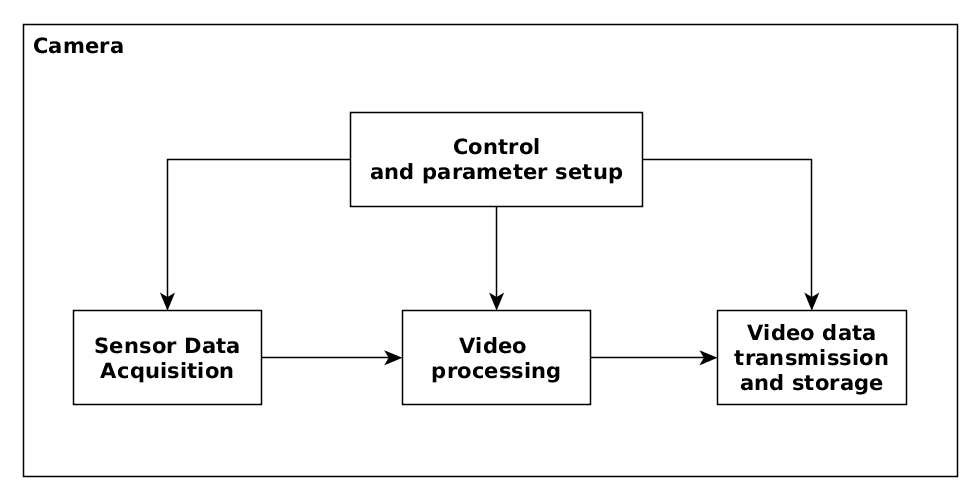
\includegraphics[width=13cm]{img/introduction/func_blk_diag2.png}
%    \caption{Functional block diagram}
%    \label{fig:func_block_diag}
%\end{figure}
%%
%The main camera functions are: video acquisition, processing, setting of parameters,
%data storage and data transmission. All of those functions are performed by the electronics, software and mechanics of
%the camera. It is essential to notice that all of these parts are mandatory for any function to work. 
%\begin{itemize}
%    \item \textbf{Sensor data acquisition} - the ability to acquire the image data from the sensor. The main parameter of this
%        function is the throughput of the camera which limits the sensor resolution as well as frame rate 
%    \item \textbf{Video processing} - the ability to process the acquired image. A still image when acquired, is in an unprocessed
%        format (RAW) which needs to be encoded into a desired format like JPEG, PNG, TIFF etc.   
%    \item \textbf{Video data transmission and storage} - the process of sending the video data over a specified medium or
%        saving it on a non-volatile storage device
%    \item \textbf{Control} - the means of setting the desired parameters of every function 
%\end{itemize}
%
%%\subsection{Hardware block diagram}
%\vspace{1cm}
%
%Hardware is another aspect of a camera's architecture (figure\ref{fig:hardware_block_diag}).
%
%\begin{figure}[h!]
%    \centering
%    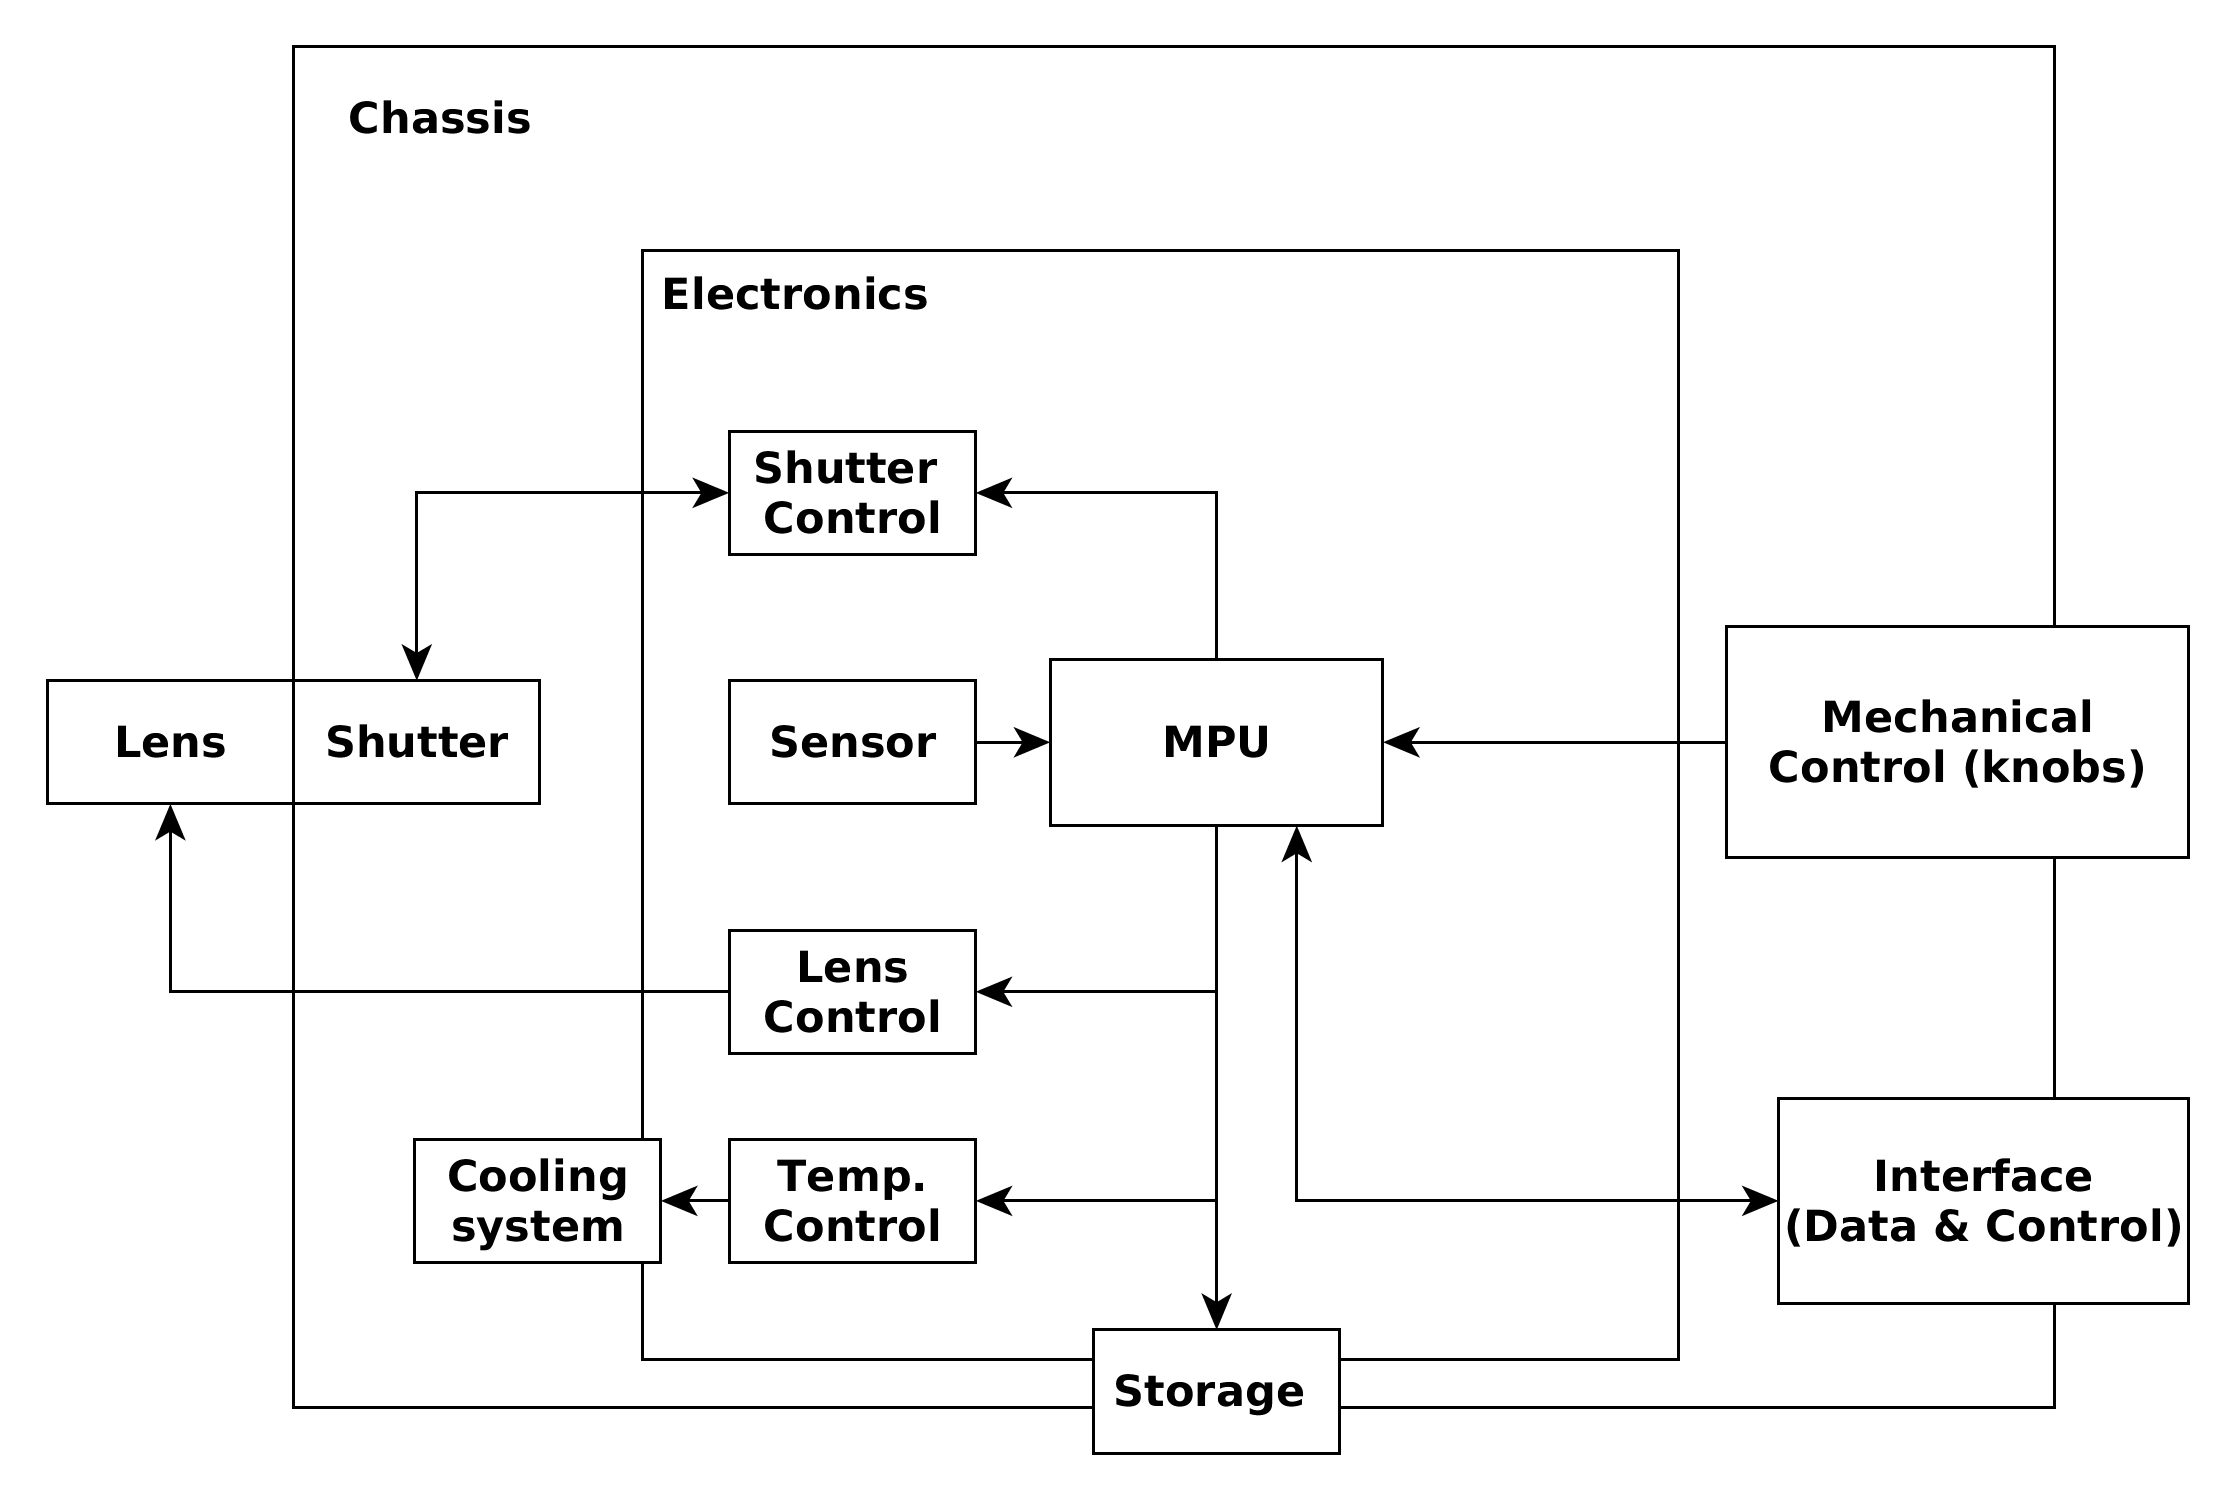
\includegraphics[width=13cm]{img/introduction/hw_blk_diag.png}
%    \caption{Hardware block diagram of a camera}
%    \label{fig:hardware_block_diag}
%\end{figure}
%
%From a hardware point of view a camera is an electro-mechanical device where the complicated mechanical systems
%have to be combined with electronics in a single chassis. The camera consists of a multitude of parts:
%\begin{itemize}
%    \item \textbf{image sensor} - a silicon integrated circuit which is photosensitive to the electromagnetic spectrum and
%        allows for capturing an image. 
%    \item \textbf{chassis} - a mechanical compartment designed to hold all the internal parts of the camera together.
%    \item \textbf{shutter} - a mechanical iris used for controlling the exposure time of the camera.
%    \item \textbf{lens} - (or system of lenses) an optical device used for focusing the light onto a sensor.
%    \item \textbf{electronics} - a dedicated embedded system used for video data acquisition and control of camera
%        parameters.
%    \item \textbf{viewfinder} - (electronic or optical) a means of viewing the acquired image before capturing -
%        directly through the lens or using the sensor.
%\end{itemize}
%
%The electronic system is another key element of the camera. It contains a dedicated silicon sensor as well as a Main
%Processing Unit (\gls{MPU}), which is usually placed on the same Printed Circuit Board (\gls{PCB}), making the design 
%difficult. On top of this, cameras use batteries as a power supply so the whole embedded system power budget has to be taken into
%account. 
%
%%\subsection{Software block diagram}
%The last aspect of camera architecture is the software. It is not uncommon for a commercial handheld camera to
%support features like automatic exposure setup, noise correction or face recognition.
%These functions are possible to achieve due to the complex software that runs inside the camera Main Processing Units. 
%Figure~\ref{fig:software_block_diag} presents the basic software architecture of a digital camera. 
%
%
%\begin{figure}[h!]
%    \centering
%    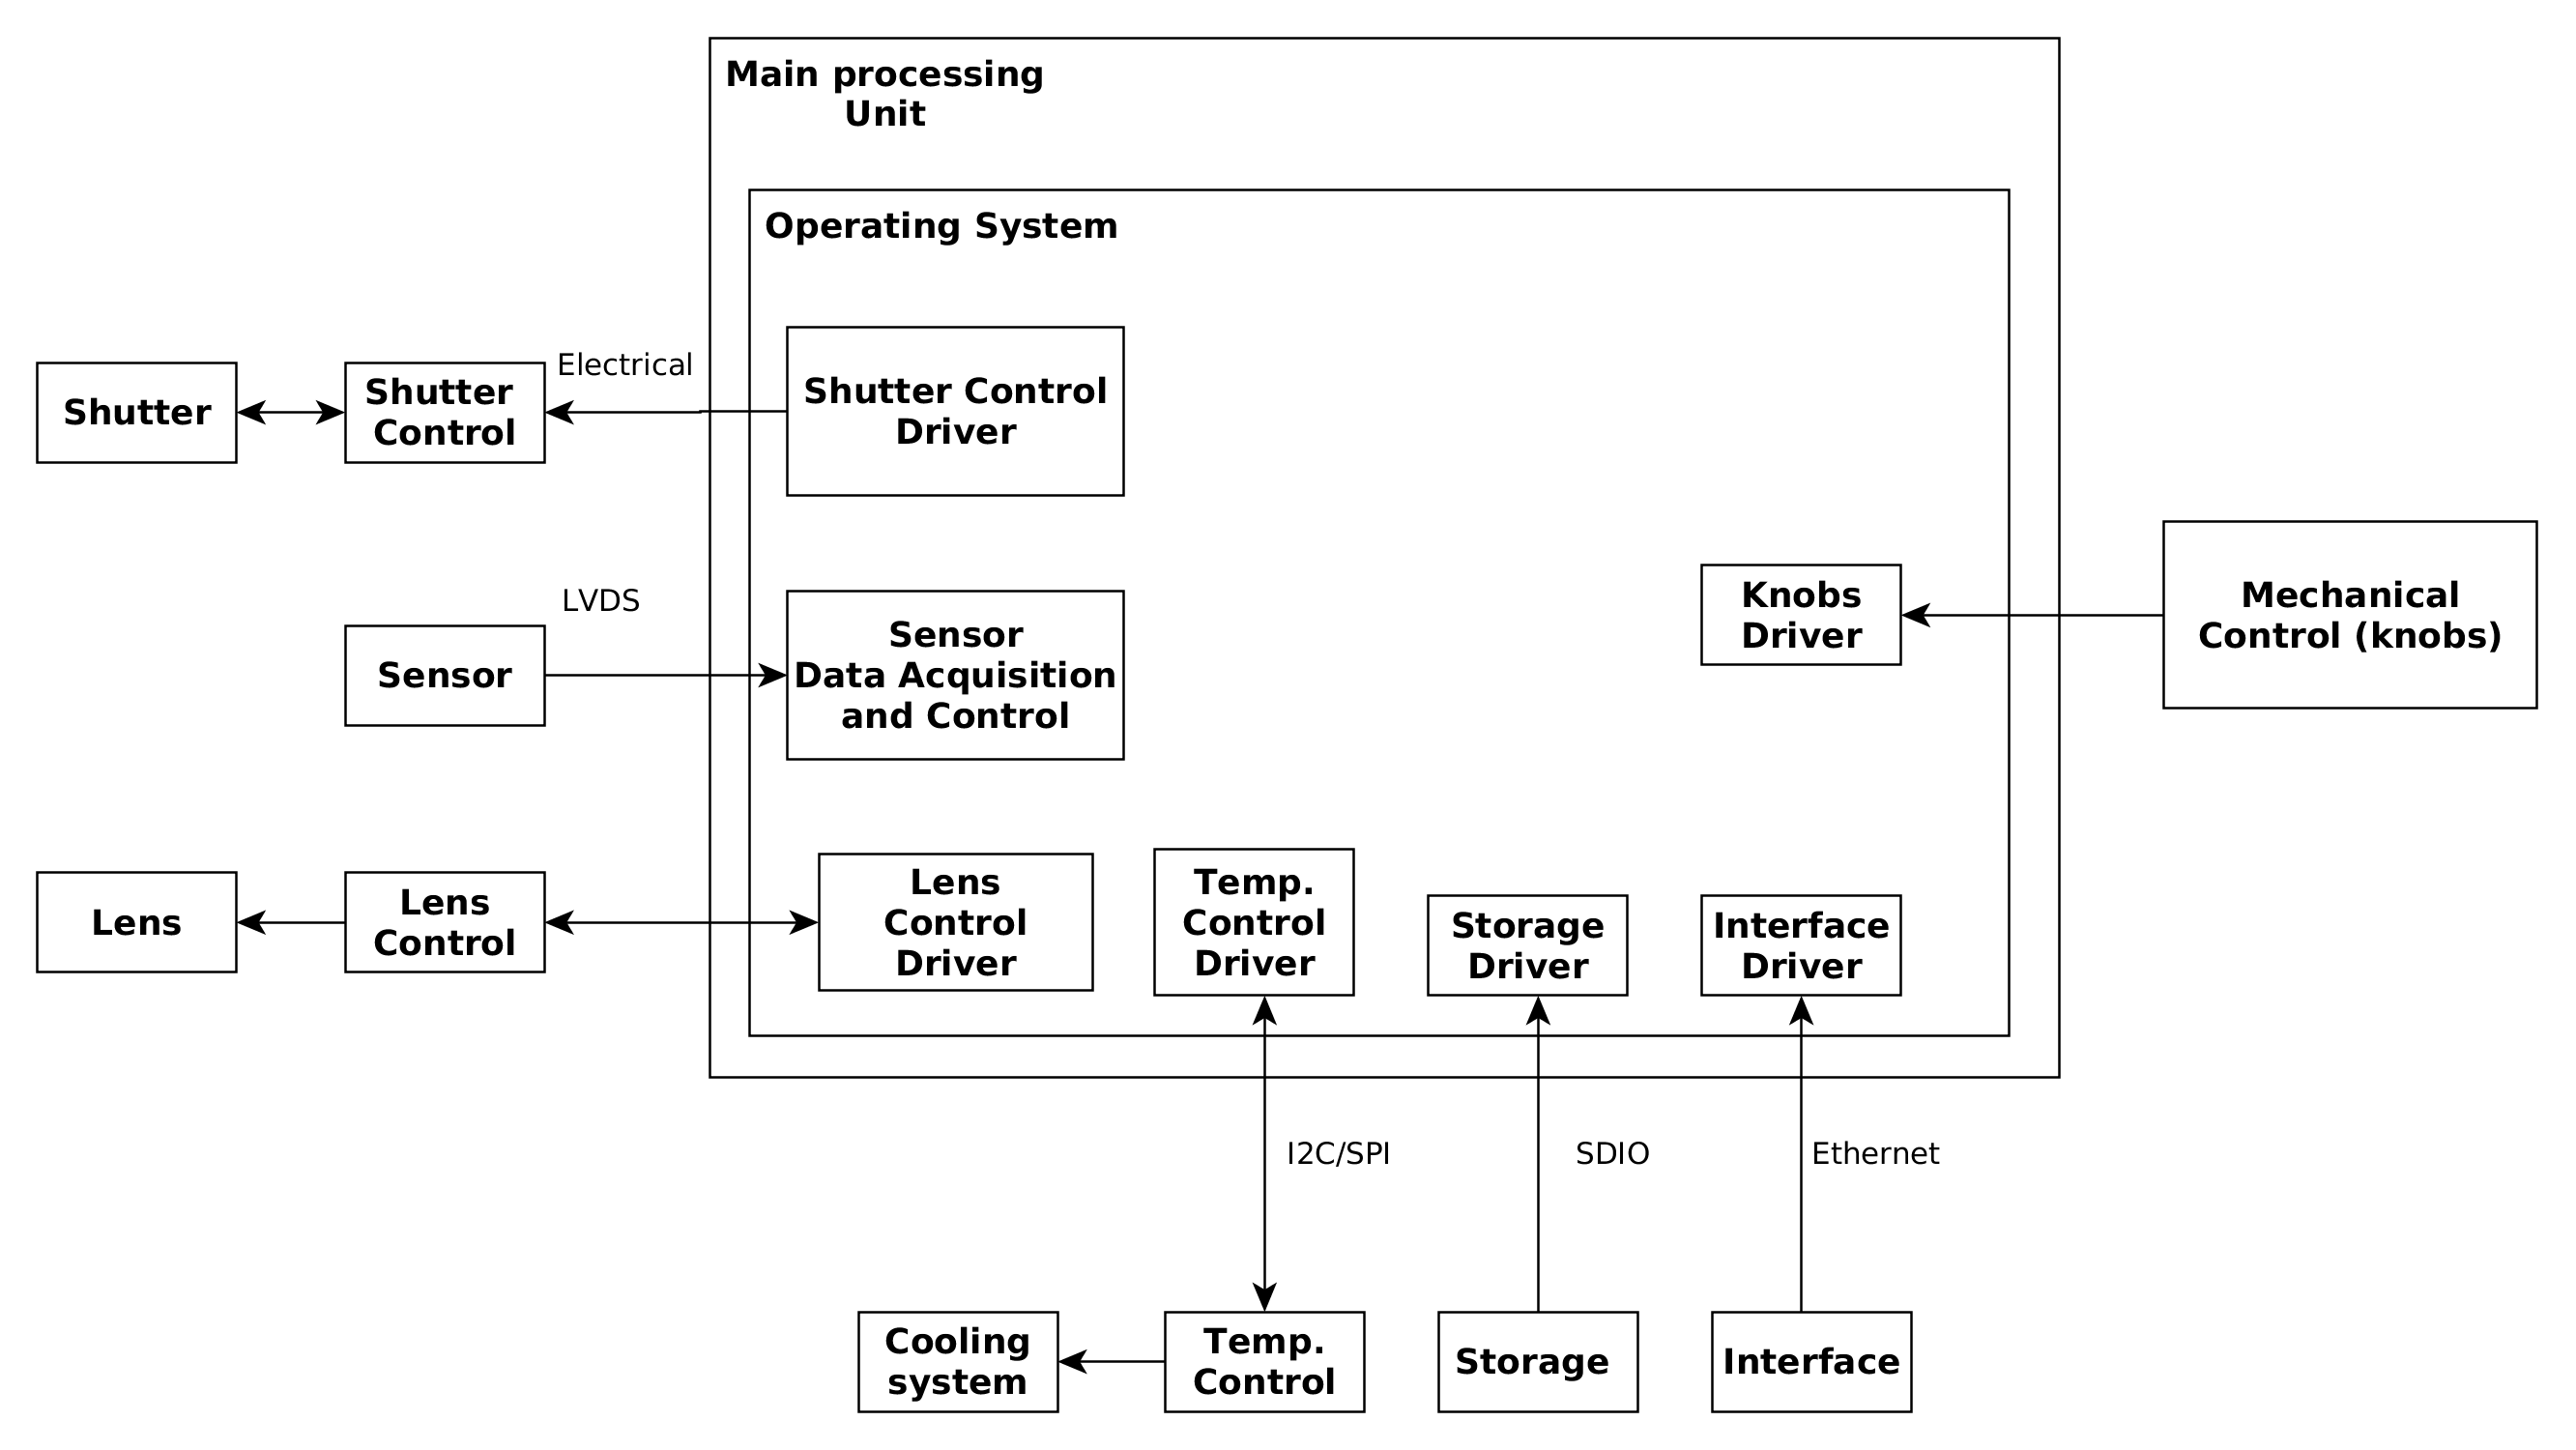
\includegraphics[width=15cm]{img/introduction/sw_blk_diag.png}
%    \caption{Software block diagram of a camera}
%    \label{fig:software_block_diag}
%\end{figure}
%
%
%The Main Processing Unit is responsible for controlling all aspects of the embedded system, including sensor data 
%acquisition and control of parameters. Depending on the type of camera software, the architecture 
%can differ significantly. 
%
%The typical software architecture of a camera consists of an operating system and dedicated drivers to perform the following
%functions:
%
%\begin{itemize}
%    \item Sensor control
%    \item Shutter control
%    \item Video data transmission 
%    \item Optics control
%    \item Data storage 
%    \item Setup of parameters 
%\end{itemize}
%
%Scientific cameras can use a real-time operating system, which is useful in performing
%synchronised acquisition with multiple channels. Specialised systems usually provide more sophisticated software to
%perform specific tasks which are not needed in commercial applications.    
%
%
%
%\subsection{Video parameters}
%
%\subsubsection{Frames per second}
%The FPS\footnote{Frames Per Second} represent the number of frames that can be acquired by a camera one after
%another during 1s. This number depends on the resolution of the sensor, throughput of storage device, and on
%the parameters of the taken pictures (exposure time).  
%
%\subsubsection{Resolution}
%Resolution is a parameter of the sensor and presents the effective number of pixels.
%Figure~\ref{FIG:RESOLUTION_COMP} presents the comparison of different resolutions of sensors. 
%They are measured in \emph{Megapixels} (MP). 
%
%
%\begin{figure}[h!]
%    \centering
%    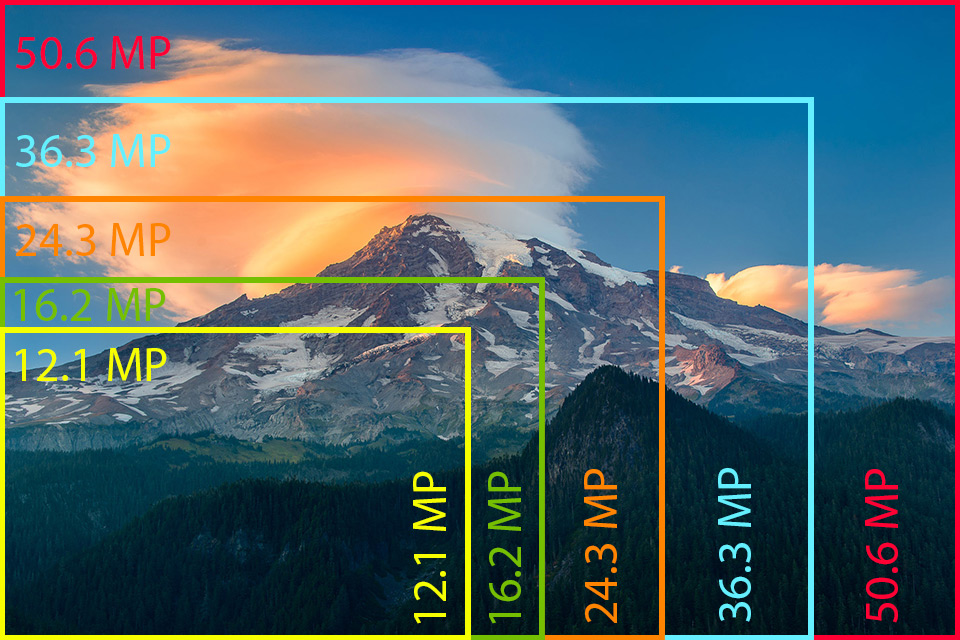
\includegraphics[width=12cm]{img/introduction/Sensor-Resolution-Comparison.jpg}
%    \caption{Sensor resolution comparison}
%    \label{FIG:RESOLUTION_COMP}
%\end{figure}
%
%
%\subsubsection{Compression}
%The acquired image from the sensor is in a pure RAW format, which means that the frame data are unprocessed and
%uncompressed. Inexpensive commercial cameras are usually unable to save a picture in this format due to its
%large size. DSLR\footnote{Digital Single Lens Reflection} cameras can save a picture in RAW format and in a
%compressed version. The typical file formats are: JPEG, PNG, TIFF, BMP.
%
%The compression degrades the picture quality, but allows for storing more images on the same storage device; this also 
%applies to video data acquisition. When the camera acquires the stream of data, it automatically
%compresses it and transfers it through a certain interface. 
%
%\subsubsection{Exposure time}
%Exposure time, or shutter speed, is the time when the light reaches the sensor. The more light that comes, the 
%higher the exposure. Figure~\ref{FIG:EXPOSURE_COMP} presents the influence of the exposure time
%on the image. As can be seen in the image the exposure time is defined as $ X^{-1} $ of a second, where $X$
%is the number representing the division factor. 
%
%
%\begin{figure}[h!]
%    \centering
%    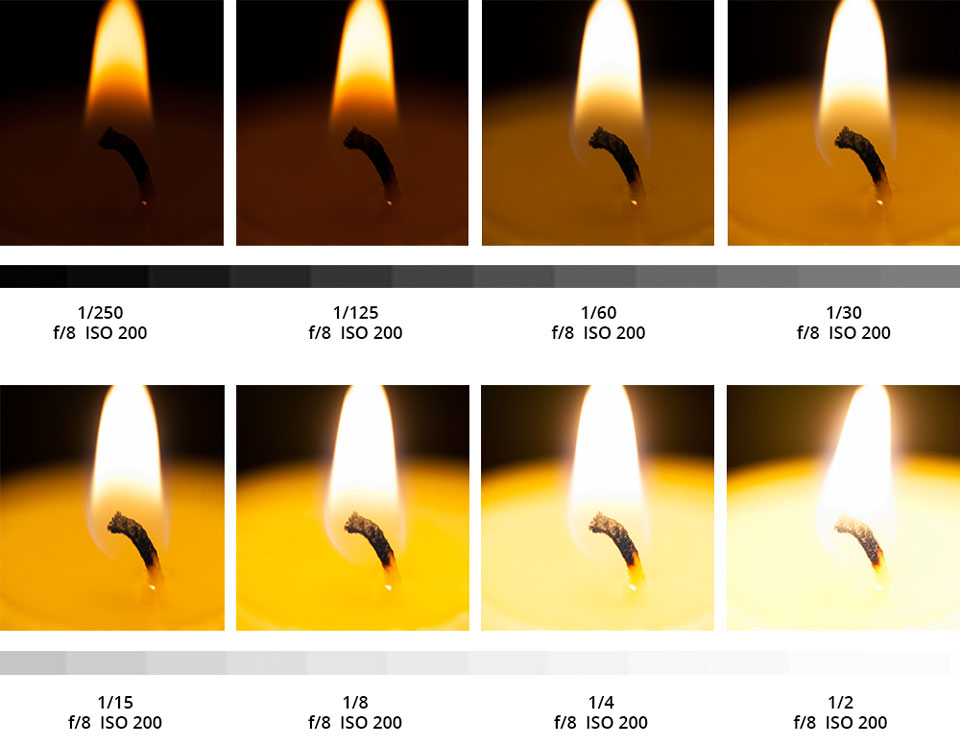
\includegraphics[width=10cm]{img/introduction/exp_time.jpg}
%    \caption{Exposure time comparison~\cite{WWW:EXP_TIME}}
%    \label{FIG:EXPOSURE_COMP}
%\end{figure}
%
%When it comes to scientific cameras, the exposure times can be long or short depending on the application. High speed
%cameras require that the exposure time is as short as possible, whereas astronomical cameras need
%high exposure times. 
%
%\subsubsection{Sensitivity - ISO}
%Another key parameter of a camera's video acquisition is the sensor's sensitivity. It is defined by an
%ISO\footnote{International Standards Organisation} parameter.  
%Figure~\ref{FIG:ISO} presents the influence of a different sensitivity on the picture. 
%
%\begin{figure}[h!]
%    \centering
%    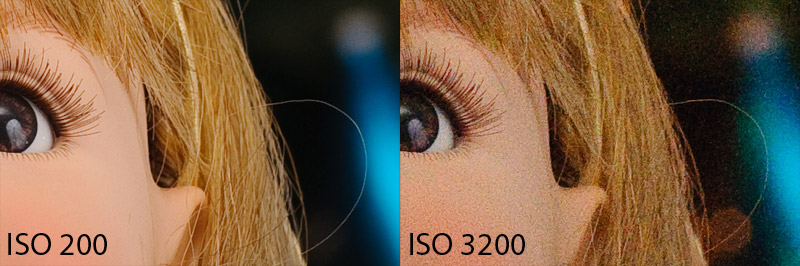
\includegraphics[width=13cm]{img/introduction/iso.jpg}
%    \caption{Influence of sensitivity (ISO) on a picture~\cite{WWW:ISO}}
%    \label{FIG:ISO}
%\end{figure}
%
%The higher the sensitivity is, the brighter the picture but higher the noise. 
%The sensitivity of an acquired picture in commercial cameras is set by the standard menu on the
%device's screen, whereas in scientific applications the process is much more complex due to the fact that it depends
%solely on the type of sensor. Some sensors (CMOS) have build-in amplifiers that make it possible to change 
%the gain of the amplification circuit, whereas the other does not have them and the gain can be only set by changing the gain
%of Analogue Front End readout. 
%
%\subsubsection{Readout noise}
%The acquired picture is not an exact representation of the reality. Ideally, each photon hitting a pixel would be converted into one electron. Then the exact
%measurement of the number of electrons should be made. Unfortunately, there are processes at each step that
%add noise to the measurement. Noise is a variation in pixel values that degrades the picture.
%
%Sensor manufacturers measure and report the noise as a number of electrons RMS (Root Mean Square).  It is typically
%presented as e.g. $15e^{-}$ RMS, meaning that with this sensor, it is expected to see about 15 electrons of
%noise per pixel.  More precisely, $15e^{-}$ RMS is the standard deviation around the mean pixel value.
%More information regarding the noise can be obtained in the literature.~\cite{WWW:NOISE} 
%
%%     In an ideal world, every photon striking a pixel would be converted into exactly one electron.  Then the number of
%%     electrons would be precisely counted and converted to a number telling the photographer exactly how much light
%%     struck each pixel.  Unfortunately, the process of converting light to pixel values in a sensor is
%%     governed by some fundamental physical laws and other factors that introduce “noise” into an image.  Noise is
%%     unwanted variations in pixel values that make the image a less than exact representation of the original scene. 
%%
%%     Noise in CCD images can manifest itself in multiple ways, including “graininess” in darker background areas, faint
%%     horizontal or vertical lines that become visible in low signal areas of the image, blotchy gradients between darker
%%     and lighter regions in a nebula, a gradient from dark to light from one corner or side of an image to the other,
%%     and especially as low contrast images — the result of a reduced signal to noise ratio. 
%%
%%     If each pixel in a CCD can hold 90,000 electrons and the average noise of the system is 30 electrons per pixel, the
%%     dynamic range, or Signal to Noise Ratio (SNR) is 90,000 / 30 or 3,000 to 1 (70db).  If the average noise can be
%%     reduced to just 15 electrons, you have effectively doubled the dynamic range to 76db, or 6,000 to 1 (90,000 / 15).
%%     Reducing the noise in CCD images is critical to producing clear, high dynamic range images. 
%
%
%%\subsection{Mechanics}
%%The mechanics in any camera design is a crucial element. It holds the electronics together with the sensor
%%and optics. Very often mechanical design include sophisticated shutter mechanism, optical 
%%stabilisation and cooling systems. The latter is frequently used in scientific cameras, where the CCD
%%sensor has to be cooled down in order to achieve lower noise levels~\cite{WWW:NOISE}. 
%%
%%\subsubsection{Chassis}
%%The camera chassis is usually made out of aluminium, magnesium or polymer. Depending on the requirements for the camera
%%operation it may conform to specific standards such as MIL-STD-810G~\cite{WWW:MIL} or IP67/IP68~\cite{WWW:IPCODE}. 
%%
%%\subsubsection{Shutter}
%%The camera shutter (\ref{FIG:SHUTTER}) is a complicated mechanical device used for closing and opening the area in front of the sensor which
%%blocks or allows for light to come through. There are two main types of shutters: leaf shutter and focal-plane
%%shutter. The first one is usually mounted within a lens, whereas the second is mounted near the focal
%%plane\footnote{focusing point of the optics, close to the sensor}. 
%%
%%\begin{figure}[h!]
%%    \centering
%%    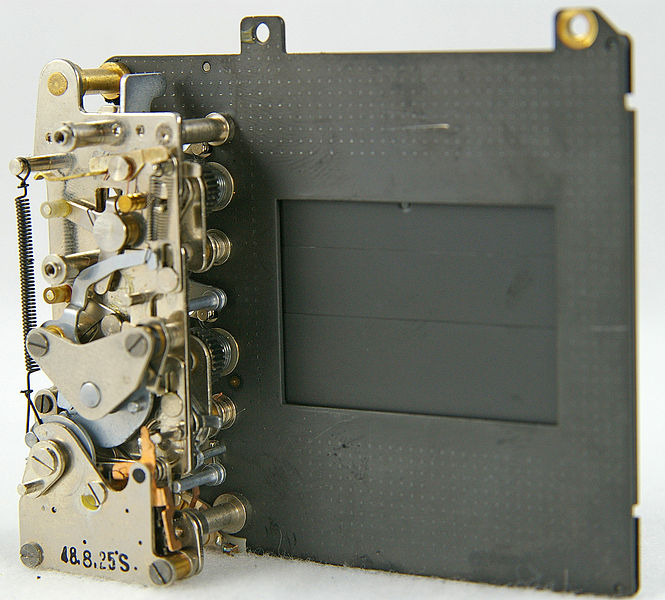
\includegraphics[width=10cm]{img/introduction/shutter.jpg}
%%    \caption{Focal-plane shutter~\cite{PIC:SHUTTER} of a DSLR}
%%    \label{FIG:SHUTTER}
%%\end{figure}
%%
%%\subsubsection{Optics}
%%Optics are one of the most important parts of a camera. Their purpose is to focus light directly at a sensor. The quality of
%%lens has an immense influence on the quality of the acquired picture. Optics usually consist of a lens which is,
%%in fact, a system of lenses with different parameters, and a diaphragm which allows for changing the aperture.    
%%
%%\begin{figure}[h!]
%%    \centering
%%    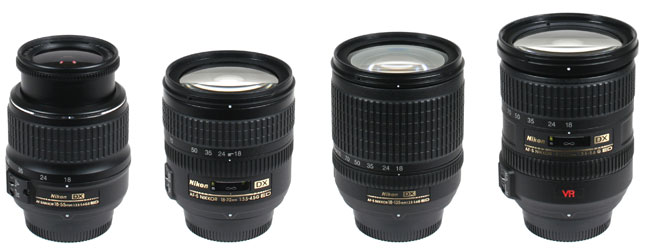
\includegraphics[width=13cm]{img/introduction/lens.jpg}
%%    \caption{Nikkor lens ~\cite{LENS}}
%%    \label{FIG:LENS}
%%\end{figure}
%%
%%There are two main parameters which describe the optical lens focal length and aperture. 
%%The focal length is the distance between the lens and the sensor when the subject is in focus, usually stated in mm,
%%whereas the aperture is the size of the diaphragm opening in the sensor which determines how much light enters the lens 
%%
%%Together they determine the optical cone of incoming light that is being focused on the sensor.  
%%
%%The quality of the lens is extremely important in order to acquire a good quality image, mainly due to optical defects which
%%happen in the lens when light is travelling through it. The better the lens the less evident the defects.  
%%Some of the main optical defects are listed below:
%%
%%\begin{itemize}
%%    \item{chromatic aberration} failure of lens to focus all the colors which result in distorted colors.
%%    \item {vignetting} physical distortion resulting in the darkening of the corners of a picture with respect to the
%%        center. 
%%    \item optical aberration - usually radially symmetric irregularity of the image's physical distances and relationships
%%        between the points in the image, e.g. barrel distortion~\ref{FIG:BARREL_DIST}. 
%%    \item spherical aberration - inability to focus light on one point, resulting in an unfocused image. 
%%    \item defocus - distortion resulting in an improperly focused image.
%%\end{itemize}
%%
%%\begin{figure}[h!]
%%    \centering
%%    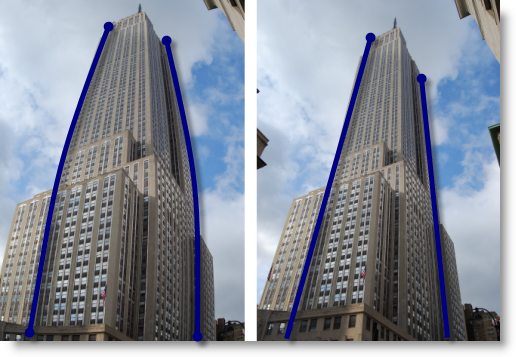
\includegraphics[width=13cm]{img/introduction/barrel.png}
%%    \caption{Barrel distortion~\cite{WWW:BARREL}}
%%    \label{FIG:BARREL_DIST}
%%\end{figure}
%%
%%
%%\subsubsection{Mounts}
%%There are a number of lens mounts for the cameras on the market. It is a mechanical and often at the same time electrical
%%interface between the camera body and the lens. Lenses can be divided into three groups: bayonet mount, breech-lock and screw-threaded
%% depending on the way the lens is attached to the body of the camera.
%%
%%The most common one is the bayonet mount, due to the fact that it can properly align the lens mechanically and
%%electrically. 
%%
%%The lenses designed for specific sensors present different properties when attached to different cameras. For
%%example, for APS-C size sensors, most of the lenses have a changed focal length which is called a
%%\textit{crop-factor} and acts as a constant by which the focal length has to be multiplied in order to obtain the real
%%value.   
%%
%%Every manufacturer has its own lens mount standard. Each mount provides different \textit{flange focal
%%distance}\footnote{Distance between the mounting flange and the sensor}. Some of the most common mounts are listed below. 
%%
%%%Lens mounts can be divided into professional use case
%%%and amateur. The design of optical path in the camera vary between different sensor sizes and %TODO check exactly how
%%%does the full frame lenses differ from nomral ones. They should have wider area of focus in comparison to DX lenses.  
%%\begin{itemize}
%%    \item \textbf{M42} - Full-frame (35 mm) lens mount, created in 1949, used on Pentax, Practica, Zeiss and Zenit cameras   
%%    \item \textbf{Nikon F} - standard Nikon lens mount used on all SLR cameras 
%%    \item \textbf{Canon EF} - standard Canon lens mounts for full frame SLR
%%    \item \textbf{PL-mount} - Arri digital cinematic camera lens mount, currently the most popular
%%    \item \textbf{PV-mount} - Panavision lens mount used on Panaflex cameras
%%\end{itemize}
%%%M mounts
%%NIKON F
%%Konica-Minolta
%%Canon? 
%
%\subsection{Electronics}
%
%\subsubsection{Central processing unit}
%
%\paragraph{FPGA}\mbox{}\\
%
%The Field programmable Gate Array is an integrated circuit consisting of a set of logic cells, reconfigurable logic blocks,
%logic elements, and dedicated resources in a reconfigurable matrix. The main advantage of FPGAs is parallelism and
%reconfigurability. The algorithm designed in the hardware can run in parallel to anything inside the logic matrix. 
%It also allows for
%\emph{pipelining}, which is a technique used for speeding up the calculations by connecting the output of one module to
%the input of other. Novel FPGAs provide unparalleled processing capability because they have high speed IOs and multigigabit
%transceivers in one chip. What is also important is that this FPGA is relatively power efficient, which makes it possible
%to use it in an embedded device. The main companies designing FPGAs are: Altera (Intel), Xilinx, Microsemi and Lattice.
%
%
%\paragraph{SoC}\mbox{}\\
%
%System on a Chip is an integrated circuit device, which is a set of multiple IPs in one package. Each of these
%IPs\footnote{Intellectual Property} usually have a different architecture. An example of an SoC is a Xilinx Zynq SoC~\cite{WWW:ZYNQ}
%which is a combination of a dual core application processor and an FPGA or a Texas Instruments OMAP~\cite{WWW:OMAP}
%series, which contains an application processor, microcontroller for real-time tasks, and a DSP for signal processing.
%This gives an immense advantage compared to other devices, due to the fact that specific tasks can be executed on a
%specialised internal core and not on a separate device. This decreases the power consumption and eases the development
%time. 
%
%\paragraph{Application processor}\mbox{}\\
%
%AP is a specialised Integrated Circuit with high processing power and ability to run a high level
%operating system such as e.g. Linux. An example of AP is Texas Instruments AM335x~\cite{WWW:AM335}, which contains ARM Cortex-A8 core.   
%Another main distinguishing feature of APs is that they contain a MMU~\footnote{Memory Management Unit}, which is a
%sophisticated internal device that controls the access to the memory and registers inside the device. In comparison to
%microcontroller's MMU is an equivalent to MPU~\footnote{Management Protection Unit} which works in a much simpler way and
%does not allow to run a high level operating system. The high processing power and ability to run Embedded Linux makes
%the Application Processor a good choice to use in any embedded systems. Nowadays, APs evolved to be incorporated in
%SoCs,
%where they can work along a Graphics Processing Unit or a microcontroller.
%
%\paragraph{ASIC}\mbox{}\\
%
%It is not uncommon for the commercial cameras to use dedicated ICs which perform image acquisition and
%image processing much faster than Application Processors or FPGAs. Such ICs are much more expensive in production than
%General Purpose ICs, which is why they are mostly used in high volume commercial products, where the initial development
%cost of designing and producing an IC can be overtaken by product sell revenue. Camera ASICs are extremely specialised.
%An example of such a processor is Nikon's \textit{Expeed} processor~\cite{WWW:EXPEED}. Figure~\ref{FIG:EXPEED} presents the architecture on
%which this processor was based.
%
%\begin{figure}[h!]
%    \centering
%    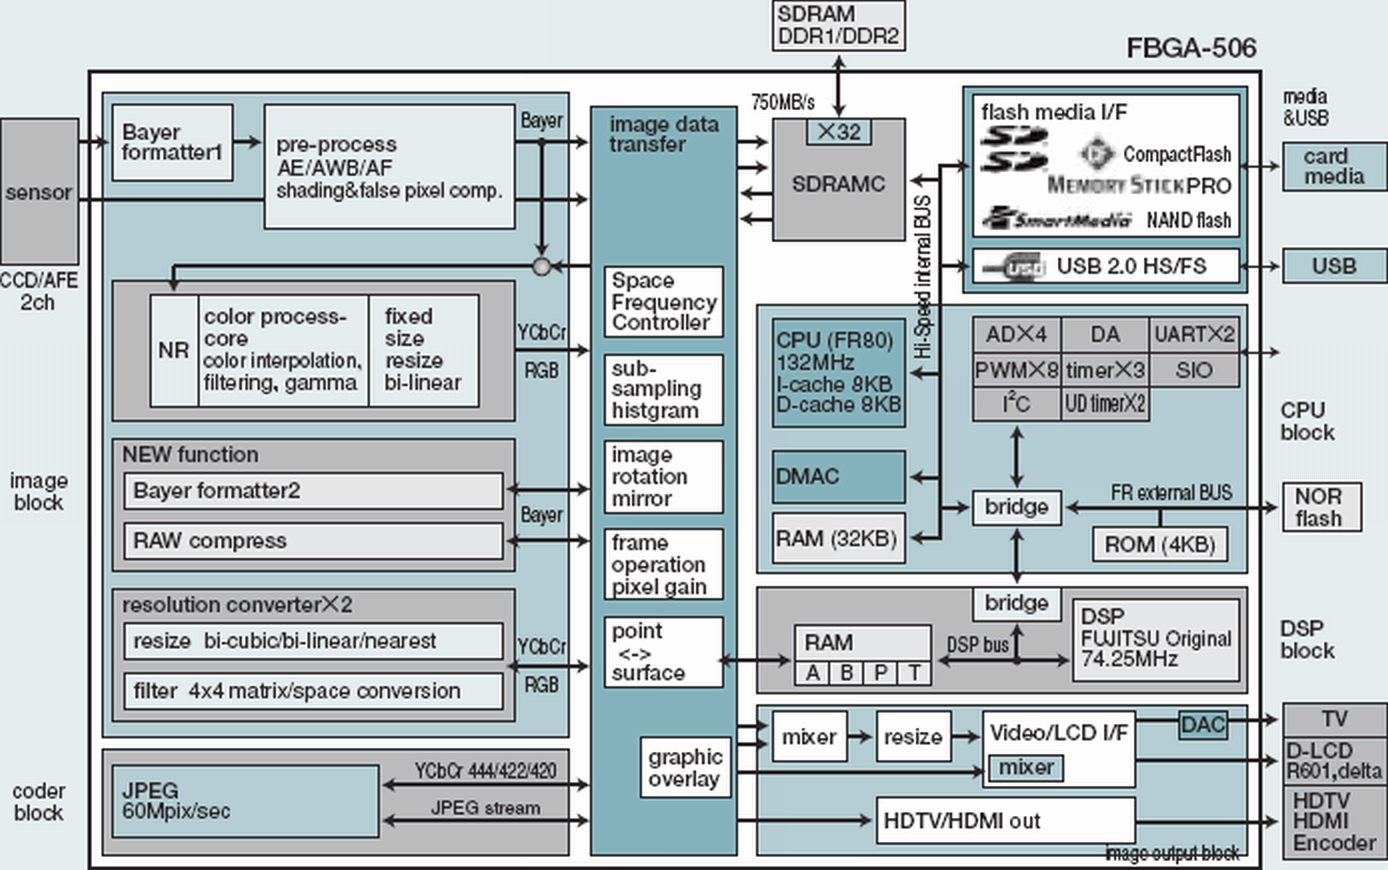
\includegraphics[width=13cm]{./img/introduction/EXPEED.png}
%    \caption{EXPEED architecture diagram~\cite{WWW:EXPEED}}
%    \label{FIG:EXPEED}
%\end{figure}
%
%The main limitation of ASICs is a lack of flexibility, since they do not provide any reconfigurability when compared to
%FPGAs. Also, depending on the architecture of the controller, they provide limited capability in terms of running an
%operating system like Embedded Linux. They are specialised chips suited for one task. They do much faster than
%before mentioned integrated circuits, but this comes with some limitations. 
%
%\subsubsection{Video data storage}
%Below, typical solutions for storage are described and both pros and cons are analysed. 
%
%\paragraph{Solid State Drive}\mbox{}\\
%
%SSD is a high throughput flash drive which uses SATA or PCIe interface. SSDs are becoming
%more and more common nowadays in any commercial device, mainly due to high speed throughput (~400-600 MB/s) and relatively high
%capacity. The main drawback of SSD is their price which is higher than for HDD, but is steadily dropping.   
%
%\paragraph{Hard Disc Drive}\mbox{}\\
%HDD are electro mechanical storage devices which are the most common medium in PC and Server
%market. This standard is being used also in cameras as a storage for videos. The main advantage is a large capacity with
%respect to size and data throughput. HDDs are also inexpensive when compared to SSDs. The major drawback
%is the weight, limited throughput (approx. 100 MB/s), high latency, and faultiness. 
%
%\paragraph{SD Card}\mbox{}\\
%SD Card (Secure Digital) is a Flash based storage method which is mostly common in inexpensive commercial handheld
%cameras, but they also, at some point become apparent in high-end cameras when the transfer speed increases. 
%The card supports SDIO (Secure Digital Input Output) interface and is commonly supported by most of the nowadays integrated
%circuits. Cards come in three different sizes: standard, mini and micro, and support up to 2 TB of data storage with a
%maximum throughput of 832 Mbps. 
%
%
%%\paragraph{Compact Flash}\mbox{}\\
%%
%%CF is a common storage medium for high-end commercial cameras. They provide a
%%high storage capacity at a reasonable price. This standard was initially more popular than SD Card and has become
%%less common in new devices. One of the reasons for this is the size of the cards which is much bigger than SD Cards. 
%%Compact Flash cards, provide high speed interface (Serial ATA or PCI Express) and
%%store up to 2 TiB\footnote{1 Tebibyte - 1024 gigibyte} of data. The standard is still being developed with the new CF 5.0 specification being
%%released soon, which increases the maximum data storage limit to 128 PB.     
%
%
%\subsection{Firmware}
%
%Firmware is responsible for numerous functions of a camera. Many incorporate application
%processors, SoC or more advanced microcontrollers. Those which do not are usually
%specialised cameras that use ASIC to acquire an image and control the functions of the device. Frequently, firmware
%is highly complicated and incorporates a digital system, low level drivers, and a high level operating systems like
%embedded Linux, Android or Windows CE.  
%
%\subsubsection{Embedded Linux}
%
%Embedded Linux is widely used in any Embedded Systems as an operating system because it is well tested,
%open, and provides numerous libraries and programs. It is not common for cameras to run Linux, except commercial
%cameras that run Android, which is based on Linux \cite{WWW:ANDROID_LINUX}. On the other hand, Linux OS is used
%in Open Source Camera projects~\cite{WWW:AXIOM_BETA} and in scientific camera research  \cite{PAPER:DYN_RECONF_CAMERA},
%\cite{PAPER:ADAS}, \cite{PAPER:ZYNQ_DETECTION} where it provides before mentioned advantages. The main disadvantage of
%Linux is that the company that uses it has to comply to numerous licenses, and also that the hardware has to be
%relatively high performance.   
%
%
%\subsubsection{Dedicated OS/Baremetal}
%
%In principle, it is not necessary for cameras to run a full fledged OS like GNU/Linux. Sometimes a dedicated OS or 
%a baremetal firmware can be used. The complexity of that system can vary from extremely simple to sophisticated custom solutions. 
%The main benefit of a dedicated OS is that it is suited specifically for a range of products, drivers can be reused
%on different types of cameras (e.g. in the same family of products) and there are no implications with the licensing, thus
%allowing for fewer errors and better customer experience. 
%
%
%%  \subsection{Software}
%%    Usually with the camera as a system for acquiring a video there is some way to control it using a PC or any other
%%    device like a smartphone for example. 
%
%\subsection{Sensors}
%
%\subsubsection{CMOS}
%%TODO add description
%The Complementary Metal-Oxide Semiconductor (CMOS) is a silicon chip technology used in electronics today. 
%The use of CMOS technology in sensor design allows for the integration of the readout and control over the pixel array directly in
%the sensor, thus simplifying the whole design process of the camera. This technology also makes the sensors less
%expensive than CCD. Image processing features can also be directly embedded into sensor which gives an immense
%advantage over the software solution, because it is faster.
%
%CMOS sensors also have some limitations when compared to CCD. One cannot achieve the same sensitivity, mainly due to the
%size of the cells, which is much smaller. A variety of CMOS sensors are used nowadays in scientific camera designs~\cite{BOOK:SCIENTIFIC_CAMERAS}. 
%
%\begin{figure}[h!]
%    \centering
%    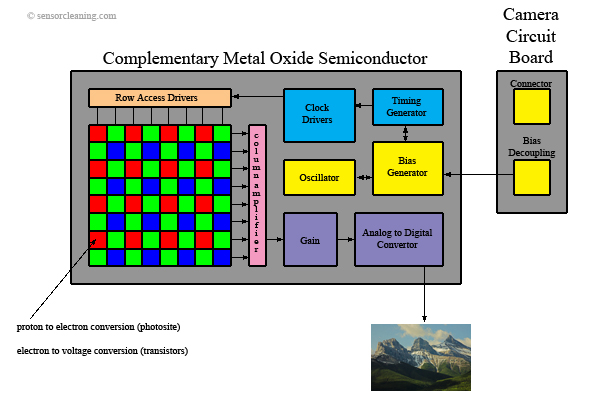
\includegraphics[width=13cm]{img/introduction/CMOS_sensor_diagram.jpg}
%    \caption{CMOS Sensor Architecture~\cite{PIC:CMOS}}
%    \label{FIG:CCD_CELL}
%\end{figure}
%
%
%\subsubsection{CCD}
%
%Charged Coupled Device (CCD) is a matrix of cells\ref{FIG:CCD}. The cells inside the CCD
%sensor are connected  to each other and create a long \emph{shift register}. During the exposure, the capacitors in
%the cells are charged. After the exposure, the charge in each cell is shifted out and sampled at the output.
%The principle is straightforward and makes it possible to achieve extremely high sensitivity pictures.
%CCD sensors can acquire images in a wide spectrum of electromagnetic wavelength~\ref{FIG:CCD_WAVELENGTH}. 
%
%\begin{figure}[h!]
%    \centering
%    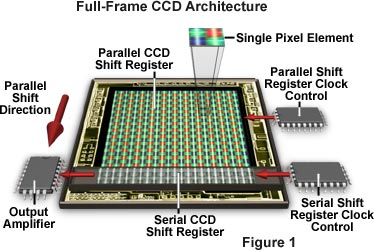
\includegraphics[width=10cm]{img/introduction/CCD.jpg}
%    \caption{CCD Sensor Architecture~\cite{PIC:CCD}}
%    \label{FIG:CCD}
%\end{figure}
%
%
%\begin{figure}[h!]
%    \centering
%    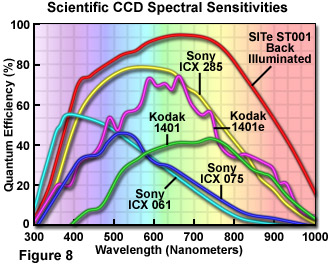
\includegraphics[width=10cm]{img/introduction/ccd_wavelength.jpg}
%    \caption{CCD Sensor wavelength sensitivity~\cite{PIC:CCD_WAVELENGTH}}
%    \label{FIG:CCD_WAVELENGTH}
%\end{figure}
%
%
%\paragraph{Light sensitivity}\mbox{}\\
%
%The sensitivity of a camera sensor is measured by: Quantum Efficiency (QE) which is \textit{a measure of
%how efficiently a sensor converts light (photons) to charge (electrons)}\cite{WWW:QE} and Read Noise (RN) which is
%\textit{a noise level (measured in electrons RMS) at the output of the sensor in the dark and at zero integration time}. 
%This value is conceptually similar to \textbf{SNR}\footnote{Signal to Noise Ratio}. 
%
%The Read Noise is greatly influenced by a number of factors like: \emph{Dark Current} which is a current that builds
%up in the CCD capacitors due to leakage. This is an especially difficult problem in astronomy applications, where pictures
%of the night sky are taken with long exposure times.  
%
%% describe whether this is different for CMOS and CCD 
%
%The phenomena decreasing the sensor sensitivity can be mitigated by a number of techniques. For example Dark Current,
%influence can be measured by taking a picture of the same exposure time as desired with a closed shutter. By doing this,
%a dark frame can be acquired and then deducted from the desired frame. 
%
%
%\subsubsection{Sensor interfaces}
%\label{ch1:sensor_interfaces}
%Silicon image sensors provide different interfaces for data transfer and control.
%The most common interfaces found in modern sensors are described in this part. 
%
%\paragraph{CSI - Camera Serial Interface}\mbox{}\\
%
%Camera Serial Interface is a serial interface used in many sensors for sending data and controlling the sensor by a host
%processor. The standard was defined by the MIPI (Mobile Industry Processor Interface) alliance, and there are three revisions
%of the standard: CSI-1, CSI-2 and CSI-3. The interface uses 6 pins to transfer data and allows for 2.5 Gbps data rate
%for CSI-2 and 5.0 Gbps for CSI-3. Serial interface also embeds I2C control bus (on separate lines), which is usually used for controlling
%the sensor. The serial interface provides high throughput, lower power consumption and easier design in any embedded
%system\cite{WWW:CSI_MIPI}.   
%
%\paragraph{CPI - Camera Parallel Interface}\mbox{}\\
%
%Camera Parallel Interface is an older data interface used for transferring data between a sensor and a host processor.
%The interface uses parallel bus architecture, where data words are sent on a separate line and an I2C
%communication interface is added, which allows for control of the sensor. The data bus consists of an 8 bit wide data
%bus and clock and synchronisation signals (vertical and horizontal).
%
%\begin{figure}[!h]
%    \centering
%    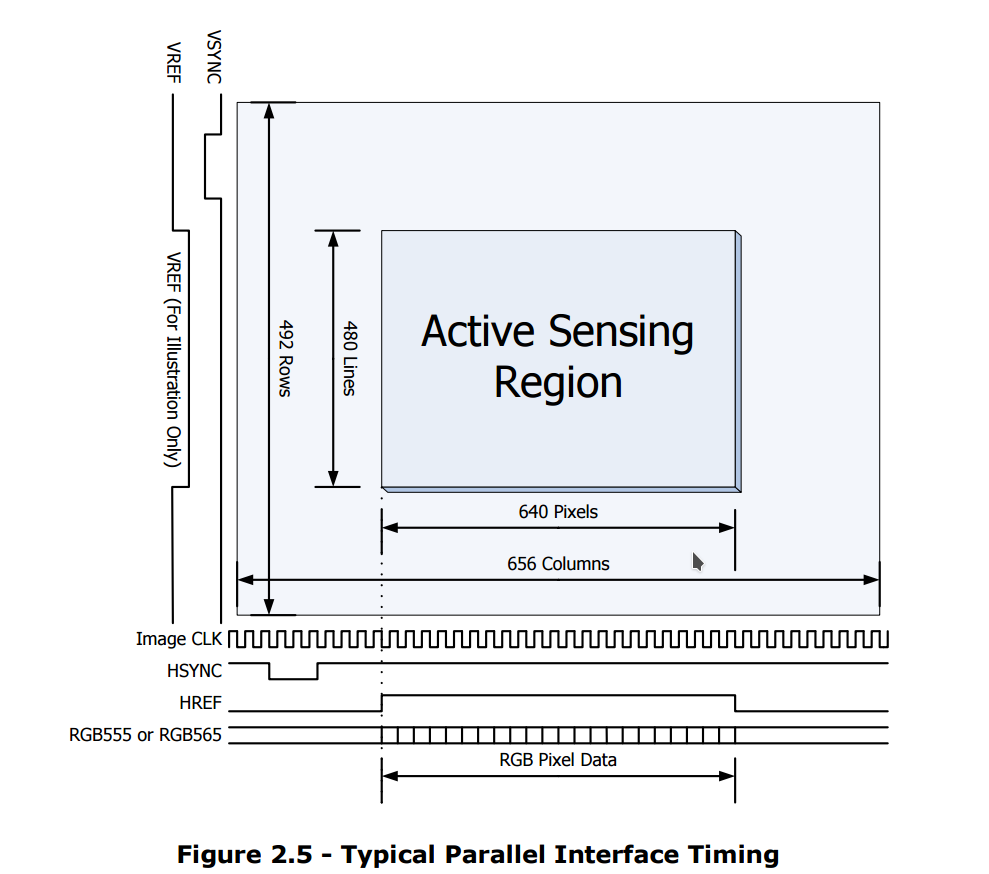
\includegraphics[width=10cm]{img/introduction/cpi.png}
%    \caption{Camera Parallel Interface data transfer diagram\cite{WWW:CPI}}
%    \label{FIG:CPI}
%\end{figure}
%
%\paragraph{Custom serial interfaces}
%
%\subsection{Camera Data Interfaces}
%The interface of the camera is another crucial aspect of the whole system. Depending on the application, cameras can provide
%different interfaces suited for different needs. The main difference is between industry and scientific cameras and
%consumer devices. For the first set, the reliable and long distance means of communication have to exist on the camera,
%whereas in a consumer product, a typical interface, like what can be found in PCs are usually incorporated. 
%
%Cameras can be divided into two groups: streaming cameras and cameras with an embedded storage medium. Additionally, even
%the cameras with internal storage need to have the data transferred at some point to another device.  
%
%The following list provides the most common interfaces that can be found in the camera systems:
%\begin{itemize}
%    \item \textbf{USB - Universal Serial Bus}\cite{WWW:USB} - a serial interface providing high throughput (up to 10 Gbps for USB 3.0) with a
%        maximum distance of 3 meters without having the need to use repeaters. USB is an extremely common interface and
%        can be found in basically every PC and embedded system nowadays. In the aspect of camera design, the 
%        limitation is the maximum distance that the data can be reliably sent, while on the other hand it is perfectly suited
%        for commercial devices to transfer data between the camera and the PC. 
%
%    \item \textbf{Ethernet - IEEE 802.3}\cite{WWW:ETHERNET} - a network serial interface, commonly used in industry and
%        commercial products. It allows for high
%        throughput long distant communication. Depending on the protocol, it requires a quite powerful processor to
%        handle the communication (TCP), precisely the stack. Some protocols like UDP are less complicated, and can be
%        implemented even in FPGA devices, which makes the interface more flexible. Additionally, one can use either
%        copper based cabling or fibre optics which can greatly increase the noise immunity and maximum measurement
%        distance. The protocol supports speeds up to 10 Gbps for conventional devices, per link. There are special video
%        interfaces based on top of Ethernet for the camera systems like GigE Vision \cite{WWW:GIGE}.
%
%    \item \textbf{Camera Link}\cite{WWW:CAMERA_LINK_INFO} - This is a serial communication protocol designed especially for camera systems and aimed to
%        standardise the communication in scientific and industrial cameras. It uses a special
%        connector which uses 28 pins to transfer serial data from the camera to the host. There
%        are three major configurations of the interface: base, medium and full. The base one supports transfer rates of
%        up to 255 MB/s whereas the full version can send even 850 MB/s. The standard uses differential pairs to send
%        data and additional signals for the synchronisation.  
%%
%%        \begin{figure}[h!]
%%            \centering
%%            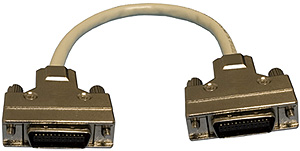
\includegraphics[width=8cm]{img/introduction/cameralink.jpg}
%%            \caption{Camera Link cable~\cite{WWW:CAMERA_LINK}}
%%            \label{FIG:CAMERA_LINK}
%%        \end{figure}
%%
%
%    \item \textbf{Wireless Field - WiFi}\cite{WWW:WIFI} - is a wireless interface used by some cameras to send video data
%        out. Wireless interface is used by the industrial camera systems or commercial ones. Wi-Fi has limited 
%        bandwidth up to 1 GbE and is prone to electromagnetic interference. There are multiple systems which provide an easy way to stream video data
%        using either Wi-Fi or any other network based interface (e.g. gstreamer\cite{WWW:GSTREAMER}). 
%
%    \item \textbf{FireWire IEEE1394}\cite{WWW:FIREWIRE} - a serial bus interface used for multimedia and video devices. 
%        It uses a serial link to transfer data for a distance up to 4.5 meters with a standard cable or up to 100 meters
%        with a coaxial or optical cable. The maximum achievable transfer rate, for the most common version of the interface 
%        S800, is 800 Mbps, and is faster than USB 2.0. The cable also provides power to the devices. 
%        FireWire is a peer-to-peer interface and allows for high-speed communication between two devices.  
%
%\end{itemize}
%
%
%\section{Specification of scientific cameras}\label{ch1:scient_theory}
%As stated before, scientific cameras are different from commercial ones in many aspects. They host different features
%and have much better performance. Usually the scientific camera is designed to do one specific task. The main 
%feature is either a dedicated custom sensor or an ability to perform custom processing embedded in the device. 
%
%%\subsection{Features}
%%
%%\paragraph{Extremely low noise}
%%%TODO add description
%%TODO
%%
%%\paragraph{Binning}
%%%TODO add description
%%TODO
%%
%%\paragraph{Multichannel operation}
%%%TODO add description
%%TODO
%%
%%\paragraph{Image processing}
%%%TODO add description
%%TODO
%
%\subsection{Existing devices on the market}
%\label{ch1:existing}
%
%\subsubsection{Elphel camera}
%Open Source camera systems an Elphel Inc. and Apertus~\cite{WWW:APERTUS} are currently the most advanced.
%Both organizations work on Open Source and Open Hardware camera systems. Elphel provided multiple cameras in the
%past, but now the only models available on the market are Elphel 353~\cite{WWW:ELPHEL_353} and the soon to be released
%Elphel 393~\cite{WWW:ELPHEL_393}. Figure~\ref{FIG:ELPHEL} present the 353 model. 
%
%
%\begin{figure}[!h]
%    \centering
%    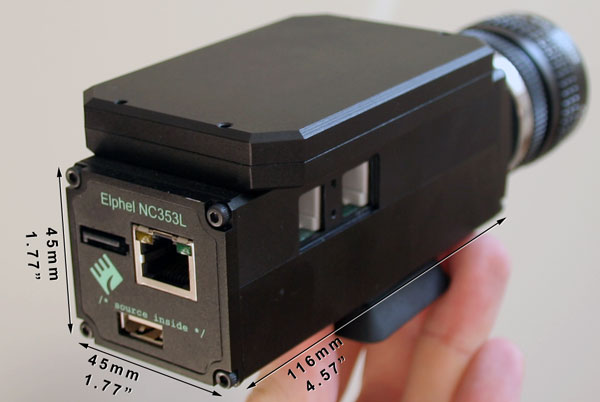
\includegraphics[width=10cm]{img/introduction/elphel_353.jpg}
%    \caption{Elphel 393 Camera}
%    \label{FIG:ELPHEL}
%\end{figure}
%
%The main parameters of the Elphel 353 model are:
%\begin{itemize}
%    \item Interfaces: SATA, Ethernet, USB, RS232
%    \item Sensors: Aptina 5MPix, Kodak 11MPix, Kodak 16MPix 
%    \item Lens mount: C-mount 
%    \item FPGA - Spartan 3e 1200K gates 
%    \item CPU - Axis ETRAX FS (200 MHz) 
%    \item 48 V DC power supply over PoE\footnote{Power over Ethernet}, 3.3 V DC input, 12-36 V DC input
%    \item Maximum power consumption 5800 milliwatts (streamer on, HD and USB flash writing at full speed)
%    \item Storage: HDD or Compact Flash
%\end{itemize}
%
%The camera was used as a module for stereography camera (360 degree camera) used in Google Maps~\cite{WWW:GOOGLE_MAPS}. 
%A newer version, which is still under development is supposed to provide higher resolutions and frame rate. 
%The project is being provided with GNU General Public License and the hardware is available with 
%CERN OHL\footnote{Open Hardware License} v1.1.
%
%\subsubsection{Apertus Axiom}
%
%Axiom Beta~\cite{WWW:AXIOM_BETA} is a camera used for the Open Cinema project. The goal is to provide a high
%performance camera and whole (software and hardware) for movie makers. The main parameters of the Axiom Beta model are:
%
%%\begin{figure}[!h]
%%    \centering
%%    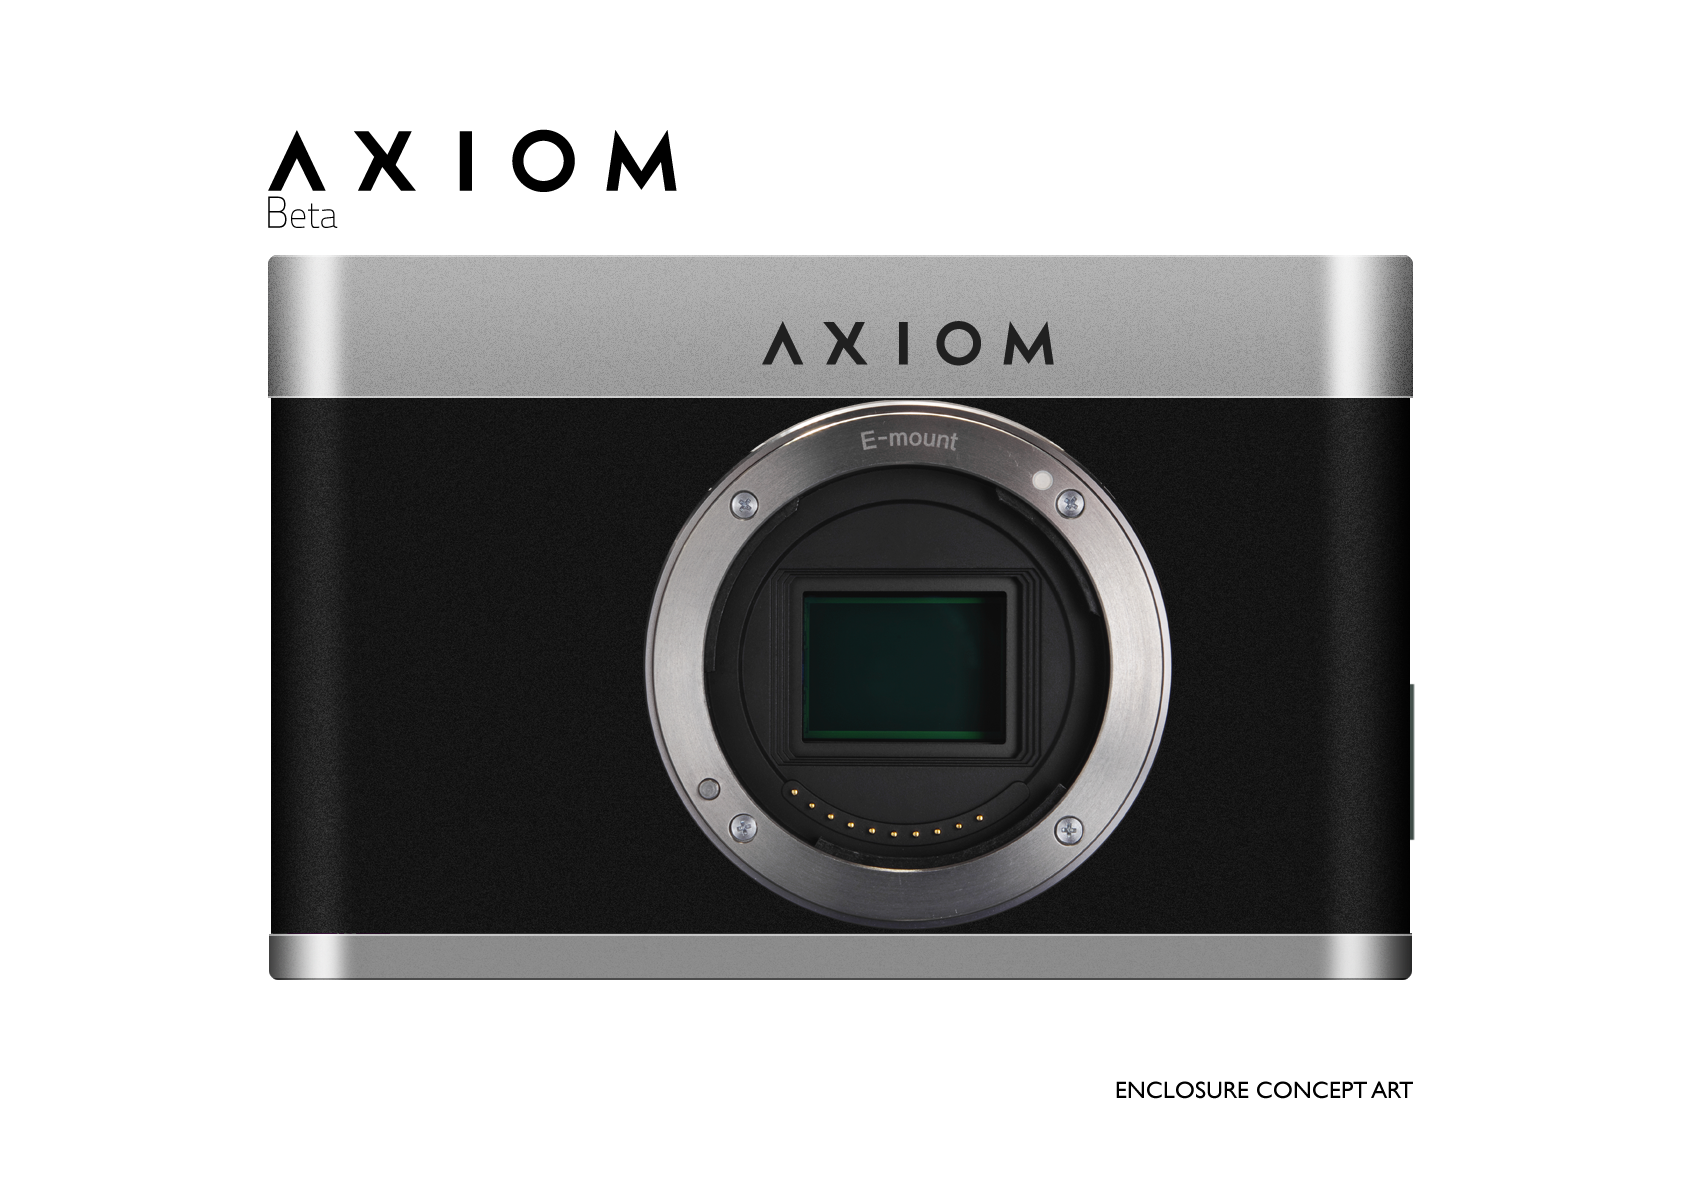
\includegraphics[width=13cm]{img/introduction/axiom_beta.jpg}
%%    \caption{Axiom Beta concept camera}
%%    \label{FIG:AXIOM_BETA}
%%\end{figure}
%
%\begin{itemize}
%    \item Interfaces: HDMI
%    \item Sensors: Kodak 11MPix, CMOSIS CNV12000, CMOSIS CNV2000 
%    \item 4K RAW experimental HDMI output over 1080p60
%    \item Lens mount: passive E-mount, passive Nikon F-mount, passive Canon EF Mount, passive M4/3 mount 
%    \item Main Processing Unit: Xilinx Zynq SoC Z7020
%\end{itemize}
%
%The camera is still under development, but current design resources are available~\cite{WWW:AXIOM_GITHUB}.
%
%\subsubsection{Atik}
%Atik is a company which specialises in the design of Astronomy Cameras.   
%As an example, an Atik 1100 camera has been chosen. It is a CCD camera that incorporates a Kodak KAI11002 sensor
%(37.25mm x 25.70 mm). It can be mounted to a telescope lens and allows for capturing astrological photos with extremely
%low noise. 
%
%Technical specification:
%
%\begin{itemize}
%    \item Sensor Type: CCD - Kodak KAI 11002
%    \item Sensor size: 37.25mm x 25.70mm
%    \item Horizontal Resolution: 4008 pixels
%    \item Vertical Resolution: 2672 pixels
%    \item Pixel Size: 9 uM x 9 uM
%    \item ADC: 16 bit
%    \item Readout Noise: 13 e- RMS typical value
%    \item Dark current: 0.03 electrons per sec at -20 degrees
%    \item Well depth: 60,000 electrons
%    \item Anti blooming: >1000x
%    \item Quantum Efficiency: 50%
%    \item Linearity: R squared test equal to 1
%    \item Interface: USB 2.0 High Speed
%    \item Power: 12v DC
%    \item Maximum Exposure Length: Unlimited
%    \item Minimum Exposure Length: 1/1000 s
%    \item Guide Port: ST-4 compatible
%        %    \item Cooling: Two stage Peltier with ΔT=-38°C, with optional water assist Full temperature regulation.
%    \item Weight: 990g
%\end{itemize}
%
%Price range is approximately 5000-6000 USD Dollars. 
%
%\begin{figure}[!h]
%
%    \centering
%    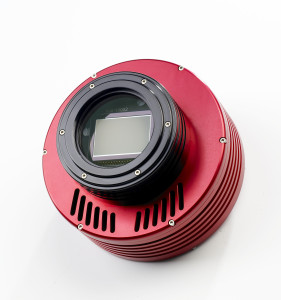
\includegraphics[width=10cm]{img/introduction/atik_camera.jpg}
%    \caption{Atik 1100 Camera}
%    \label{FIG:ATIK}
%
%\end{figure}
%
%
%%\paragraph{Hammamatsu}
%%%TODO add description
%
%
%%\subsection{Literature study}
%
%\subsection{Current research}
%Nowadays, there is a significant amount of research carried out in the topic of camera designs. FPGAs and
%SoCs integrated circuits started becoming more commonly used as the Main Processing Units for real-time video processing. 
%This provides a substantial advantage when compared to ASICs or x86 software-based approaches.  
%
%Dynamic Partial Reconfiguration\cite{PAPER:DYN_RECONF_CAMERA} in a FPGA based camera to
%provide additional functionality to a video processing pipeline which can be reconfigured on the fly even during
%operation by using a PCAP\footnote{Processor configuration access port}. The results of the research clearly shows the advantages of 
%using an advanced SoC which combine Application Processor with an FPGA in one single die. 
%
%What is more, with a more and more sophisticated neural network algorithms and processing capabilities of embedded systems,
%smart cameras are starting to be used in real-time image recognition in applications like autonomous cars. ADAS
%is an \emph{Advanced driver assistance system} which helps a driver in the driving process. These
%systems are extremely sophisticated and can detect road signs in real time and adjust the speed of a vehicle
%accordingly \cite{PAPER:ADAS},\cite{PAPER:OPENCV_ADAS}, \cite{PAPER:ZYNQ_DETECTION}. Research shows that by having a 
%more powerful embedded processor in SoC chip, when compared to previous solutions, allows for use in real-time video processing.  
%
%In general, reconfigurable logic devices, due to their nature and possibility to use \emph{pipelining}, are of great use
%in applications where algorithms can be parallelized. This is a case, to some extent, in image processing which results
%in the development of accelerators~\cite{PAPER:FPGA_VIS_FEATURES} for specific tasks like feature recognition or edge detection. 
%
%Another novel research in embedded cameras is the design of efficient systems which provide significant image processing
%capabilities \cite{PAPER:POWER_EFF_ARCH}, something which was not possible before in such a low power budget. 
%
%Research review provides a significant result. Almost every research group would benefit from having an already
%pre-configured camera design framework that would ease the development of a specific image recognition algorithm or
%high performance embedded system application. Unfortunately, such a framework doesn't exist.   
%
%%\cite{PAPER:UAV_CAMERA}
%%\section{Summary}
%
%
